\section{Problem Definition}
\label{mls:problem_definition}

Multi-level secure databases (referred to as \gls{mls} databases going forward) differ from traditional databases in that there is content within the database that cannot be accessed by all users of the database. There is data within the database itself that contains a high security classification (or multiple security classifications) than other data. This is also more volatile than multi-tenant systems. Multi-tenant systems also contain data which cannot be accessed by all users, but the data within the system contains the same priority when it comes to transaction scheduling. Security classifications within \gls{mls} databases introduce priorities and therefore introduce the issues of starvation. \gls{mls} databases also introduce the issue of covert channels since there are multiple security classifications. 

A covert channel is a channel of communication that performs communication outside of the normal access control mechanisms. This then makes it very hard to to secure using existing security measures since normal security measures are performed on the existing access control mechanisms. There are two main types of covert channels; storage channels and timing channels. Storage channels are a form of communication by modifying an existing storage location with data that would normally not be detected. Timing channels expose security issues by the presence or absence of a delay in transaction processing. Figure \ref{fig:covert_channel_exposure} shows the time delay difference between a normal operating system load to that of a delayed load operation. This presence of a time delay can allow for information passing to occur and the attacker to infer components of the system architecture especially in \gls{mls} databases.

\begin{figure}
\centering
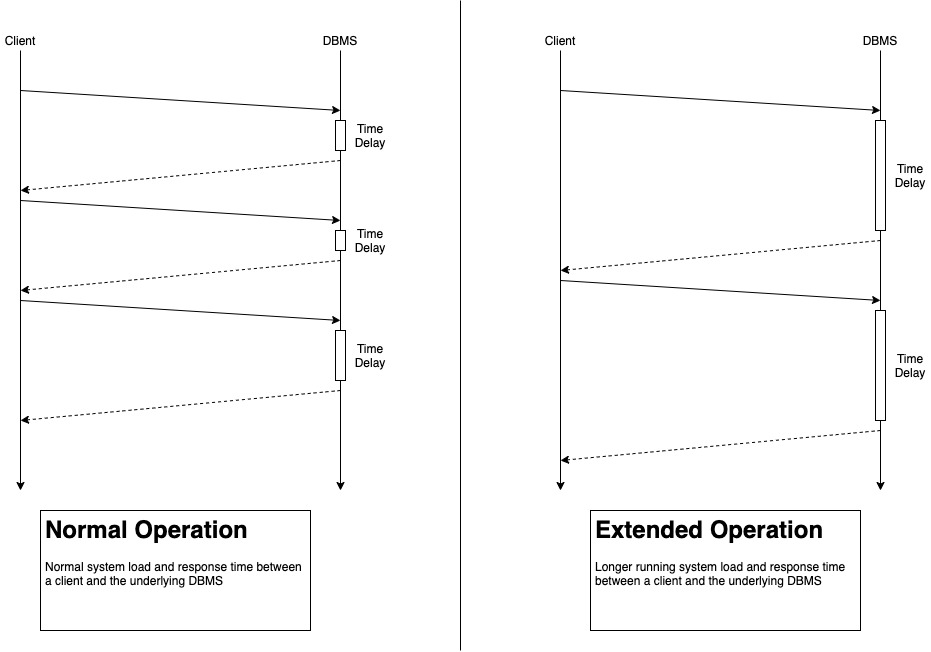
\includegraphics[scale=0.45]{images/CovertTimingChannel.jpg}
\caption{Covert Channel Exposure}
\label{fig:covert_channel_exposure}
\end{figure}

In order to prevent a timing covert channel within \gls{mls} database systems, there must not be a presence of a timing delay for transactions with lower security classifications. The transactions must incur the standard time delay as a normal transaction so that there is no suspicion that a covert channel is available.

\subsection{Elevating The Priority}
\label{mls:problem_definition_elevation}
Most concurrency control algorithms solve this issue by giving a sort of precedence or priority to lower security classification transactions to prevent any time delay. However, this can cause issues with transactions with a higher security classifications if high security transactions continually conflict with lower transactions. The high security transactions can suffer from starvation and cause a huge performance hit. Figure \ref{fig:ws_trans_starvation} shows an example of how a high security classification transaction can experience starvation with standard locking mechanisms.

\begin{figure}
\centering
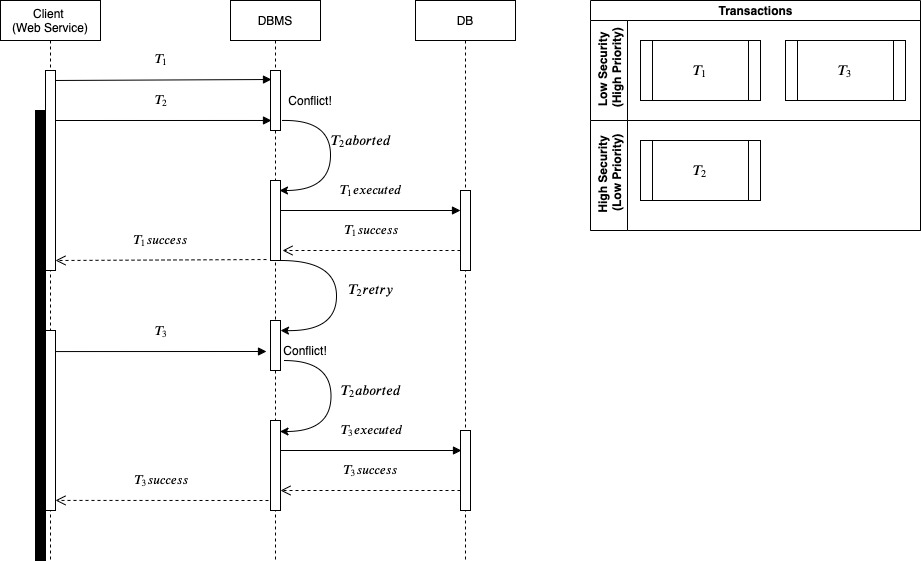
\includegraphics[scale=0.45]{images/TransactionStarvation.jpg}
\caption{Web Service Transaction Starvation}
\label{fig:ws_trans_starvation}
\end{figure}

Figure \ref{fig:ws_trans_starvation} shows an example of three transactions ($T_1$, $T_2$, and $T_3$) entering a system via a web service. $T_1$ and $T_3$ are of a low security classification while $T_2$ is of a high security classification. $T_1$ and $T_2$ enter the system at the same time and are accessing a shared resource between the two transactions. This causes a conflict and in order to prevent a timing covert channel, we abort the higher security transaction, $T_2$. $T_1$ is then able to execute successfully and complete. We then attempt to retry $T_2$ but coincidentally another transaction, $T_3$, is submitted for execution. The same process happens again, $T_2$ is aborted, and $T_3$ is executed successfully. The black vertical bar on the left side of Figured \ref{fig:ws_trans_starvation} shows the process of $T_2$ through all the aborts that happened. This illustrates the starvation of $T_2$ that happens when trying to prevent covert channels.

\subsection{Problem Identified}
\label{mls:poblem_identified}
After analyzing the system structure and architecture of an \gls{mls} database and seeing a use-case scenario, we see two problems that can be improved upon. The first being the existence of a timing covert channel due to a conflict among low and high security transactions. The second problem identified is the starvation of high security transactions due to the solution that many lock-based concurrency control algorithms present to address timing covert channels. Both of these problems have been addressed in past research (look at \cite{samarati_database_2016} for example) by simply causing transactions of a higher-security classification to abort in order to make way for the lower-security classification and then adding a priority to higher-security transactions in order to prevent starvation.

But the problem with this approach is that there is no flexibility within the solution to abort a problematic low-security transaction. The current solution leverages a binary decision model and priorities within the recovery model to address the side effect of starvation. The real problem is providing a solution that eliminates the timing covert channel with minimal side effects to efficiency and consistency that have to be reconciled. This solution would provide a safe and reliable way to abort both high-security and low-security transactions to prevent covert channels depending on the system environment.

We believe that this problem can be addressed with the dynamic categorization and reputation that the prediction-based scheduler provides in Chapters \ref{chap:prediction_based_scheduler} and \ref{chap:dynamic_reputation}.